% comment out for student version
\ifdefined\Student\relax\else\def\Teacher{}\fi

\documentclass[12pt]{article}

\title{Doubly-Linked Lists}
\author{Chris Mayfield and Dee Weikle}
\date{Summer 2021}

%\ProvidesPackage{cspogil}

% fonts
\usepackage[utf8]{inputenc}
\usepackage[T1]{fontenc}
\usepackage{mathpazo}

% spacing
\usepackage[margin=2cm]{geometry}
\renewcommand{\arraystretch}{1.4}
\setlength{\parindent}{0pt}

% orphans and widows
\clubpenalty=10000
\widowpenalty=10000
\pagestyle{empty}

% figures and tables
\usepackage{graphicx}
\usepackage{multicol}
\usepackage{tabularx}
\usepackage{wrapfig}

% fixed-width columns
\usepackage{array}
\newcolumntype{L}[1]{>{\raggedright\let\newline\\\arraybackslash\hspace{0pt}}m{#1}}
\newcolumntype{C}[1]{>{\centering\let\newline\\\arraybackslash\hspace{0pt}}m{#1}}
\newcolumntype{R}[1]{>{\raggedleft\let\newline\\\arraybackslash\hspace{0pt}}m{#1}}

% include paths
\makeatletter
\def\input@path{{Models/}{../../Models/}}
\graphicspath{{Models/}{../../Models/}}
\makeatother

% colors
\usepackage[svgnames,table]{xcolor}
\definecolor{bgcolor}{HTML}{FAFAFA}
\definecolor{comment}{HTML}{007C00}
\definecolor{keyword}{HTML}{0000FF}
\definecolor{strings}{HTML}{B20000}

% table headers
\newcommand{\tr}{\bf\cellcolor{Yellow!10}}

% syntax highlighting
\usepackage{textcomp}
\usepackage{listings}
\lstset{
    basicstyle=\ttfamily\color{black},
    backgroundcolor=\color{bgcolor},
    numberstyle=\scriptsize\color{comment},
    commentstyle=\color{comment},
    keywordstyle=\color{keyword},
    stringstyle=\color{strings},
    columns=fullflexible,
    keepspaces=true,
    showlines=true,
    showstringspaces=false,
    upquote=true
}

% code environments
\newcommand{\java}[1]{\lstinline[language=java]{#1}}%[
\lstnewenvironment{javalst}{\lstset{language=java,backgroundcolor=}}{}
\lstnewenvironment{javabox}{\lstset{language=java,frame=single,numbers=left}\quote}{\endquote}

% PDF properties
\usepackage[pdftex]{hyperref}
\urlstyle{same}
\makeatletter
\hypersetup{
  pdftitle={\@title},
  pdfauthor={\@author},
  pdfsubject={\@date},
  pdfkeywords={},
  bookmarksopen=false,
  colorlinks=true,
  citecolor=black,
  filecolor=black,
  linkcolor=black,
  urlcolor=blue
}
\makeatother

% titles
\makeatletter
\renewcommand{\maketitle}{\begin{center}\LARGE\@title\end{center}}
\makeatother

% boxes [optional height]
\newcommand{\emptybox}[1][10em]{
\vspace{1em}
\begin{tabularx}{\linewidth}{|X|}
\hline\\[#1]\hline
\end{tabularx}}

% models
\newcommand{\model}[1]{\section{#1}\nopagebreak}
\renewcommand{\thesection}{Model~\arabic{section}}

% questions
\newcommand{\quest}[1]{\subsection*{Questions~ (#1)}}
\newcounter{question}
\newcommand{\Q}{\vspace{1em}\refstepcounter{question}\arabic{question}.~ }
\renewcommand{\thequestion}{\#\arabic{question}}

% sub-question lists
\usepackage{enumitem}
\setenumerate[1]{label=\alph*)}
\setlist{itemsep=1em,after=\vspace{1ex}}

% inline answers
\definecolor{answers}{HTML}{C0C0C0}
\newcommand{\ans}[1]{%
\ifdefined\Student
    \leavevmode\phantom{~~\textcolor{answers}{#1}}
\else
    ~~\textcolor{answers}{#1}
\fi}

% longer answers [optional height]
\newsavebox{\ansbox}
\newenvironment{answer}[1][4em]{
\nopagebreak
\begin{lrbox}{\ansbox}
\begin{minipage}[t][#1]{\linewidth}
\color{answers}
}{
\end{minipage}
\end{lrbox}
\ifdefined\Student
    \phantom{\usebox{\ansbox}}%
\else
    \usebox{\ansbox}%
\fi}


\begin{document}

\maketitle

% Learning objective:
% \item Explain why Java's implementation of LinkedList is doubly-linked.

%\model{Doubly-Linked Lists}

Java's implementation of \java{LinkedList} stores two references in each node: one for the {\it previous}, and one for the {\it next}.
In addition, both the head and the tail are stored in the wrapper class.

\begin{center}
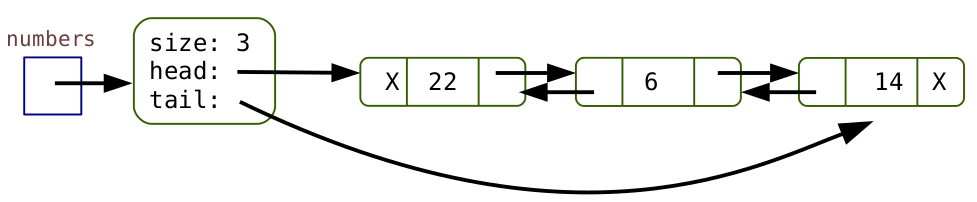
\includegraphics[scale=0.35]{doubly-linked.png}
\end{center}


\quest{10 min}


\Q How many operations are required to add an element {\it at the start} of this list?

\begin{answer}
In general, 3 operations: one to create the element, one to copy the reference to the next node, and one to change the reference from the head to the new element.
(If it's the first node, then the tail reference would also need to be set.)
\end{answer}

\Q How many operations are required to add an element {\it at the end} of this list?

\begin{answer}
In general, 3 operations: one to create the element, one to create the reference to the previous node, and one to change the reference from the tail to the new element.
\end{answer}

\Q How much memory is required for each node?
How does that amount compare with using an \java{ArrayList}?

\begin{answer}
Each element requires two references, so there is $N \times 8$ bytes of extra overhead (where $N$ is the length of the list).
\end{answer}


\Q \label{whydoubly}
What problems of singly-linked lists do doubly-linked lists solve? (In other words, what do the \java{previous} and \java{tail} make possible?)

\begin{answer}
They allow for quick access to things at the end of the list, so adding/removing at either end is fast.
They also allow for the list to be traversed backwards.
\end{answer}


%\Q Why does Java provide multiple implementations of its collection interfaces?
%
%\begin{answer}
%Each has their pros and cons; it depends on how they're being used in a program and what the most common operations will be.
%\end{answer}


\Q If your program requires a \java{List} collection, how would you decide which implementation to use? (\java{ArrayList} vs ~\java{LinkedList})

\begin{answer}
If adding items at the end and accessing random elements, use ArrayList.
If inserting items in the middle and only accessing at the two ends, use LinkedList.
\end{answer}

\end{document}
